\section{Literature study characteristics}
The literature research is performed by using the bibliographic databases Scopus and Web of Science with the following search query: \emph{("learning to rank" OR "learning-to-rank" OR "machine learned ranking") AND ("parallel" OR "distributed")}. An abstract based manual filtering step is applied where I filter those results that actually use the \emph{parallel} or \emph{distributed} terms in context to the \emph{learning to rank}, \emph{learning-to-rank} or \emph{machine learned ranking}. Studies focusing on efficient query evaluation instead of efficient model training are likely to meet all criteria listed. As a last step I will filter out studies based on the whole document that only focus on efficient query evaluation and not on parallel or distributed learning of ranking functions.\\

on Scopus the defined search query resulted in 65 documents. Only 14 of those documents used \emph{large scale}, \emph{parallel} or \emph{distributed} terms in context to the \emph{learning to rank}, \emph{learning-to-rank} or \emph{machine learned ranking}. 10 out of those 14 documents focussed on parallel or distributed learning of ranking functions.\\

The defined search query resulted in 16 documents on Web of Science. Four of those documents were also present in the set of 65 documents found using Scopus, leaving 61 unique documents. Only four of those 61 documents used \emph{large scale}, \emph{parallel} or \emph{distributed} terms in context to the \emph{learning to rank}, \emph{learning-to-rank} or \emph{machine learned ranking}, none of them focussed on parallel or distributed learning of ranking functions.\\

On Google Scholar the defined search query resulted in 3300 documents. We evaluate the first 300 search results.\\

A one-level forward and backward reference search is used to find relevant papers missed so far. To handle the large volume of studies involved in the backward and forward reference search, relevance of the studies will be evaluated solely on the title of the study. Backward reference search resulted in 10 studies regarded as potentially relevant based on the title of which four were actually relevant and included in the literature description. Forward reference search resulted in 10 potentially relevant titles, of which x studies turned out to be relevant.\\

Research in large scale Learning-to-Rank model training can be categorised according to the approach that they take in scaling up the training step of Learning-to-Rank models. Figure \ref{fig:related_work_categories} illustrates the categories of scalable training approaches in Learning-to-Rank. The following sections describe the related work in the field following the categorisation depicted in Figure \ref{fig:related_work_categories}.

\begin{figure}
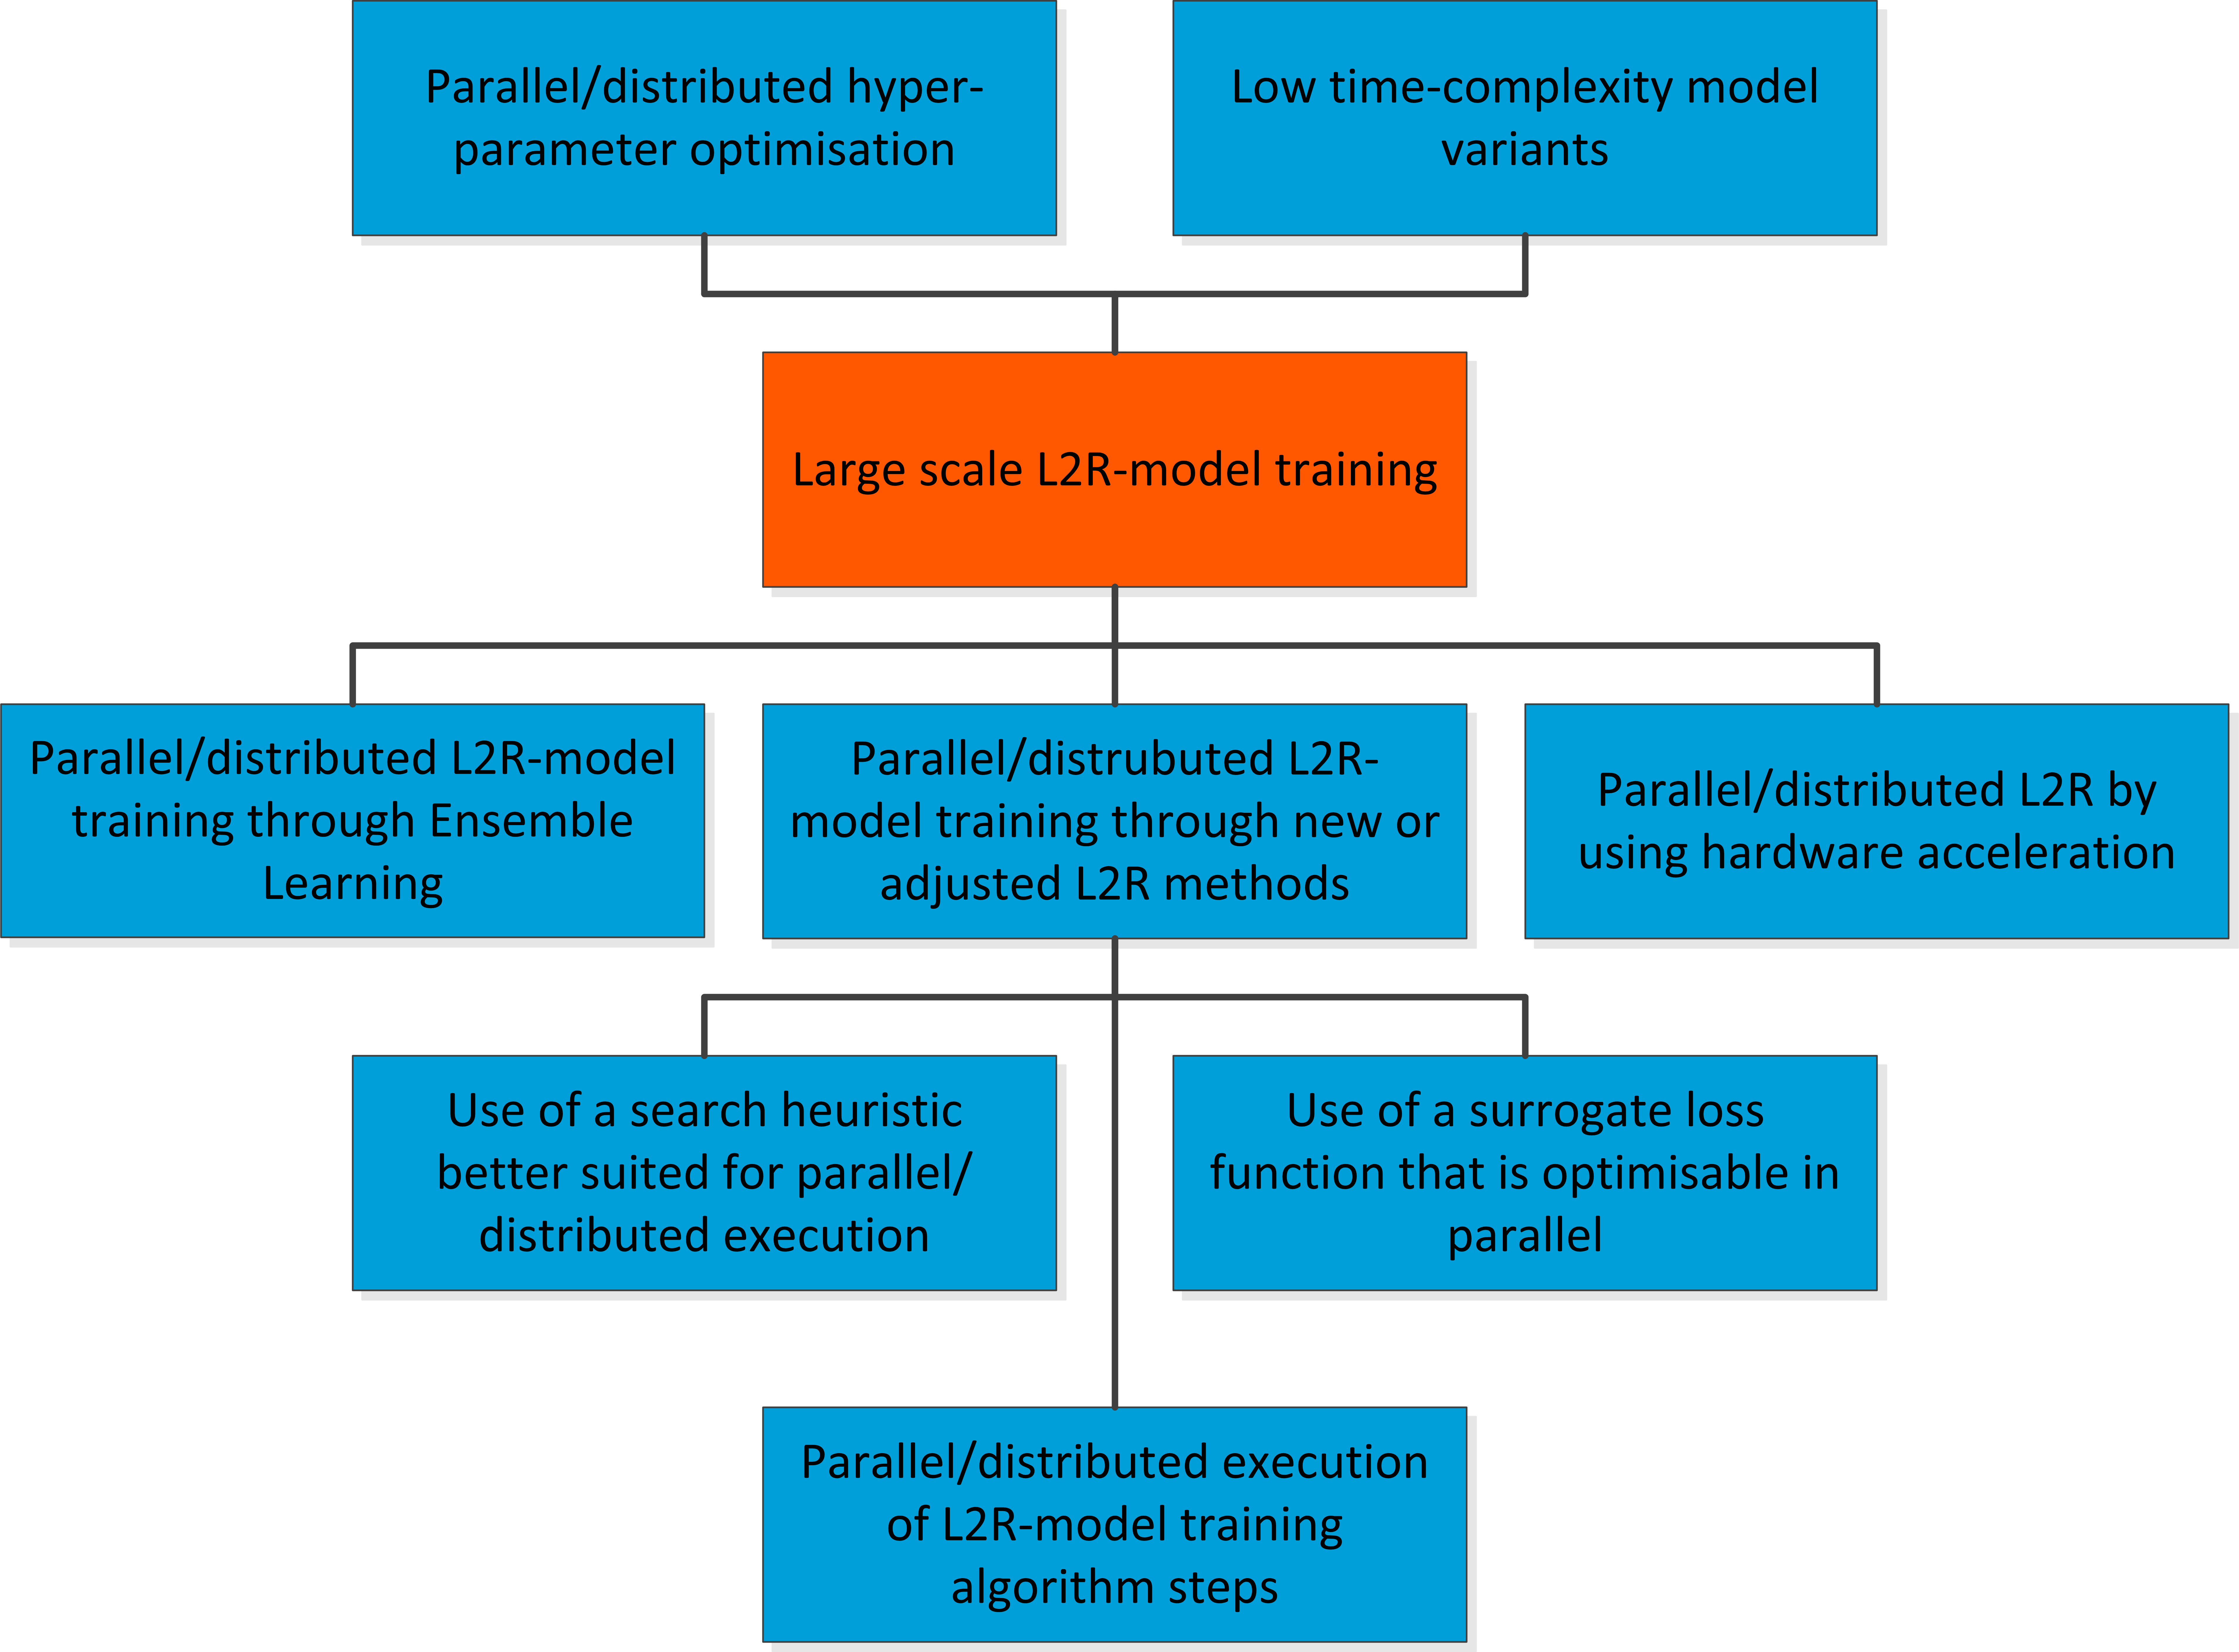
\includegraphics{gfx/related_work_categories}
\caption{Categories in research on large scale training of  Learning-to-Rank models}
\label{fig:related_work_categories}
\end{figure}

\section{Parallelising Learning-to-Rank through ensemble learning}
Schapire proved in 1990 that a strong model can be generated by combining weak models through a procedure that he called boosting \cite{Schapire1990}. The invention of the boosting method resulted in an increasing focus in machine learning research on methods to combine multiple weak models, which are called ensemble learning methods. Well-known ensemble methods include gradient boosting \cite{Friedman2001}, bagging \cite{Breiman1996}, AdaBoost \cite{Freund1997} and stacked generalisation (stacking) \cite{Wolpert1992}.\\

Ensemble methods can be used to parallelise learning methods by training the weak models in the ensemble on different nodes. In the Learning-to-Rank field parallelisation of model training through ensemble learning is frequently achieved using decision tree learners and often using the boosting ensemble method, jointly called \acf{GBDT}. \ac{GBDT}'s are shown to be able to achieve good accuracy in a Learning-to-Rank setting when used in a pairwise \cite{Zheng2007} or listwise \cite{Chen2008} setting.

\subsection{Gradient Boosting}
Gradient Boosting \cite{Friedman2001} is an ensemble learning method in which multiple weak learners are iteratively added together into one ensemble model in such a way that new models focus more on those data instances that were misclassified before.\\

Kocsis et al. \cite{Kocsis2013} propose way to train multiple weak learners in parallel by extending those models that are likely to yield a good model when combined through boosting. Authors showed through theoretical analysis that the proposed algorithm asymptotically achieve equal performance to regular gradient boosting. \ac{GBDT} models could be trained in parallel using their BoostingTree algorithm.\\

Tyree et al. \cite{Tyree2011} describe a way of parallelising \ac{GBDT} models for Learning-to-Rank where the boosting step is still executed sequentially, instead the construction of the regression trees themselves are parallelised. The parallel decision tree building is based on Ben-Haim and Yom-Tov's work on parallel construction of decision trees for classification \cite{Ben-Haim2010}. Decision trees are build layer-by-layer where the calculations needed for building each new layer in the tree are divided over the nodes using a master-worker paradigm. The data is partitioned of the workers, who compress their share into histograms and send these to the master. The master uses those histograms to approximate the split and build the next layer. The master than communicates this new layer to the workers who can use this new layer to compute new histograms. this process is repeated until the tree depth limit is reached. The tree construction algorithm parallelised with described master-worker method is \ac{CART} \cite{Breiman1984}. Speed-up experiments on the LETOR and the Yahoo! Learning to Rank challenge data sets were performed. This parallel \ac{CART}-tree building approach showed speed-up of up to 42x on shared memory machines and up to 25x on distributed memory machines.\\

Ye et al. \cite{Ye2009} described how to implement the stochastic \ac{GBDT} model in a parallel manner using both MPI and Hadoop. Stochastic \ac{GBDT} differs from regular \ac{GBDT} models by using stochastic gradient boosting instead of regular gradient boosting. Stochastic gradient boosting is a minor alteration to regular gradient boosting that, at each iteration of the algorithm, trains a base learner on a sub-sample of the training set that is drawn at random without replacement \cite{Friedman2002}. Experiments showed the Hadoop implementation to result into too expensive communication cost to be useful. Authors believed that these high communication costs were a result of the communication intensive implementation that was not well suited for the MapReduce paradigm. The MPI approach proved to be successful and obtained near linear speed-ups.\\

Svore and Burges \cite{Svore2010,Svore2012} designed two approaches to train the LambdaMART \cite{Wu2008} model in a distributed manner. Their first approach is applicable in case the whole training set fits in main memory on every node, in that case the tree split computations of the regressions trees in the LambdaMART tree ensemble are split and the data is not. The second approach distributes the training data and corresponding training computations and is therefore scalable to high amounts of training data. Both approaches achieves a six times speed-up over LambdaMART on 32 nodes compared to a single node.

\subsection{Boosting wrapped in Bagging}
Some approaches combine both boosting and bagging. Bagging \cite{Breiman1996}, also called bootstrap aggregating, is a ensemble learning method in which $m$ training sets $D_1..D_m$ are constructed from the training set $D$ by uniformly sampling data items from $D$ with replacement. The bagging method is parallelisable by training each $D_i$ with $i \in \{1..m\}$ on a different node.\\

Pavlov et al. \cite{Pavlov2010} from Yandex were the first to propose a boosting-wrapped-in-bagging approach, which they called BagBoo. The boosting step itself is not parallelisable, but the authors state that learning a short boosted sequence on a single node is still a do-able task.

Ganjisaffar et al. \cite{Ganjisaffar2011c, Ganjisaffar2011b} proposed a pairwise boosting-wrapped-in-bagging model called BL-MART, in contrast to BagBoo which is a pointwise model. BL-MART adds a bagging step to the LambdaMART \cite{Wu2008} ranking model, a model that uses the Gradient Boosting \cite{Friedman2002} ensemble method combined with regression tree weak learners. In contract to BagBoo, BL-MART is limited in the number of trees. An experiment on the TD2004 dataset resulted in 4500 trees using BL-MART while 1.1 million trees were created with the BagBoo model.

\subsection{Stacked generalisation}
% TODO: Kijken naar deze subsection, is erg zwak %
A \ac{DSN} is a processing architecture developed from the field of \emph{Deep Learning}, that uses the \ac{MSE} loss function that is easily optimisable. \ac{DSN} is based on the stacked generalization (stacking) ensemble learning method \cite{Wolpert1992}, an approach where several learning models are stacked on top of each other in such a way that the output of a model is used as one of the input features of models higher up in the stack. Each layer in the stack learns has the task of learning the weights of the inputs of that layer. The close-form constraints between input and output weights allow the input weight matrices to be estimated in a parallel manner. Deng et al. \cite{Deng2013} % TODO: beschrijven Deng et al.%\\

\subsection{Randomisation}
Most ensemble learning based Learning-to-Rank methods are based on boosting. Although boosting have shown to be an effective method in Learning-to-Rank, it has the drawback that the models in the ensemble are not completely mutually independent, which makes the process harder to parallelise. Geurts and Louppe \cite{Geurts2011} propose a tree based ensemble method in which the trees are build using random subsets of the available features. The authors called this method \ac{ET} and originally proposed this method for classification and regression settings instead of ranking settings \cite{Geurts2006}. The \ac{ET} algorithm is similar to the well-known Random Forest algorithm, with two differences: 1) in \ac{ET} each tree is build on the complete dataset instead of random subsets of the data and 2) \ac{ET} sets the discretisation thresholds that define the splits in the tree randomly, instead of based on the sample. The randomisations in the process make the models in the ensemble mutually independent, which makes it trivial to parallelise by training each tree on a different node. In contrary to what one might think, \ac{ET}s show very good performance on benchmark data with a 10th place in the Yahoo! Learning to Rank Challenge.\\

\section{Learning-to-Rank parallelisation by hardware acceleration}
Hardware accelerators are special purpose processors designed to speed up compute-intensive tasks. An \ac{FPGA} and a \ac{GPU} are two different types of hardware that can achieve better performance on some tasks though parallel computing. In general, \ac{FPGA}s provide better performance while \ac{GPU}s tend to be easier to program \cite{Che2008}. Some research has been done in parallelising Learning-to-Rank methods using hardware accelerators.

\subsection{FPGA-based parallel Learning-to-Rank}
Yan et al. \cite{Yan2009,Yan2010,Yan2011,Yan2012} described the development and incremental improvement of a \ac{SIMD} architecture \ac{FPGA} designed to run the Neural Network based LambdaRank Learning-to-Rank algorithm. This architecture achieved a 29.3X speed-up compared to the software implementation when evaluated on data from a commercial search engine. The exploration of \ac{FPGA} for Learning-to-Rank showed other advantages of the \ac{FPGA} approach next to faster model training. In their latest publication \cite{Yan2012} the \ac{FPGA} based LambdaRank implementation showed it could achieve up to 19.52X power efficiency and 7.17X price efficiency for query processing compared to Intel Xeon servers currently used at the commercial search engine.\\

Xu et al. \cite{Xu2007b,Xu2009} designed an \ac{FPGA}-based accelerator to reduce the training time of the RankBoost algorithm \cite{Freund2003}, a pairwise ranking function based on Freund and Schapire's AdaBoost ensemble learning method \cite{Freund1997}. Xu et al. \cite{Xu2009} state that RankBoost is a Learning-to-Rank method that is not widely used in practice because of its long training time. Experiments on MSN search engine data showed the implementation on a \ac{FPGA} with \ac{SIMD} architecture to be 170.6x faster than the original software implementation \cite{Xu2007b}. In a second experiment in which a much more powerful \ac{FPGA} accelerator board was used, the speed-up even increased to 1800x compared to the original software implementation \cite{Xu2009}.\\

\subsection{GPGPU for Learning-to-Rank}
Wang et al. \cite{Wang2009} experimented with a \ac{GPGPU} approach for parallelising RankBoost. Nvida \ac{CUDA} and ATI Stream are the two main \ac{GPGPU} computing platform and are released by the two main \ac{GPU} vendors Nvidia and AMD. Experiments show a 22.9x speed-up on Nvida \ac{CUDA} and a 9.2x speed-up on ATI Stream.\\

De Sousa et al. \cite{DeSousa2012} proposed a \ac{GPGPU} approach to improve both training time and query evaluation through \ac{GPU} use. An association rule based Learning-to-Rank approach proposed by Veloso et al. \cite{Veloso2008} has been implemented using the \ac{GPU} in such a way that the set of rules van be computed in parallel, in different threads, for each document. A speed-up of 127X in query processing time is reported based on evaluation on the LETOR dataset. The speed-up achieved at learning the ranking function was unfortunately not stated.\\

\section{Parallelised execution of algorithm steps in Learning-to-Rank methods}
Some research focused on parallelising the steps Learning-to-Rank algorithms that can be characterised as strong learners.
\subsection{Parallel ListNet using Spark}
Shukla et al. \cite{Shukla2012} explored the parallelisation of the well-known ListNet Learning-to-Rank method using Spark. Spark is a parallel computing model that is designed for cyclic data flows which makes it more suitable for iterative algorithms. Spark is incorporated into Hadoop since Hadoop 2.0. The Spark implementation of ListNet showed near a linear training time reduction.\\

\section{Low complexity Learning-to-Rank}
\label{sec:related_work_low_complexity}
Designing Learning-to-Rank algorithms with low time complexity for training is another approach towards large scale Learning-to-Rank. Pahikkala et al. \cite{Pahikkala2009} describe a pairwise \ac{RLS} type of ranking function, RankRLS, with time complexity $\mathcal{O}(n^3+n^2m)$, with $n$ the number of features and $m$ the number of training documents. The RankRLS ranking function showed ranking performance similar to RankSVM \cite{Herbrich1999, Joachims2002} on the BioInfer corpus \cite{Pyysalo2007}, a corpus for information extraction in the biomedical domain.\\

Lee and Lin \cite{Lee2014} describe a lower time complexity method to train a linear kernel RankSVM \cite{Herbrich1999, Joachims2002}. The authors observed that linear kernel RankSVMs are inferior in accuracy compared to nonlinear kernel RankSVMs and \ac{GBDT}s and are mainly useful to quickly produce a baseline model. Details of the lower time complexity version of the linear kernel RankSVM will not be discussed as it is shown to be an inferior Learning-to-Rank method in terms of accuracy.\\

\section{Parallelisable Search Heuristics for Listwise ranking}
Direct minimisation of ranking metrics is a hard problem due to the non-continuous, non-differentiable and non-convex nature of \ac{nDCG}, \ac{ERR} and \ac{MAP}. This optimisation problem is generally addressed either by replacing the ranking metric with a convex surrogate, or by heuristic optimisation methods such as Simulated Annealing or a \ac{EA}. One \ac{EA} heuristic optimisation method that is successfully used in direct rank evaluation functions optimisation is the \ac{GA} \cite{Yeh2007}. \ac{GA}s are search heuristic functions that mimic the process of natural selection, consisting of mutation and cross-over steps \cite{Holland1995}. The following subsection describe related work that uses search heuristics for parallel/distributed training.
\subsection{Immune Programming}
Wang et al. \cite{Wang2009b} proposed a \ac{IP} solution to direct ranking metric optimisation and observed that all \ac{EA}s are generally easy to implement such that it can be carried out on different computers distributively. However, no statements on the possible speed-up of a distributed implementation of the \ac{IP} solution has been made and no speed-up experiments have been conducted.
\subsection{CCRank}
Wang et al. \cite{Wang2011a,Wang2011b} propose a parallel evolutionary algorithm based on \ac{CC}, a type of evolutionary algorithm. The \ac{CC} algorithm is capable of directly optimizing non-differentiable functions, as \ac{nDCG}, in contrary to many optimization algorithms.  the divide-and-conquer nature of the \ac{CC} algorithm enables parallelisation. CCRank showed an increase in both accuracy and efficiency on the LETOR 4.0 benchmark dataset compared to the baselines. It must be stated however that the increased efficiency was achieved through speed-up and not scale-up. Two reasons have been identified for not achieving linear scale-up with CCRank: 1) parallel execution is suspended after each generation to perform combination in order to produce the candidate solution, 2) Combination has to wait until all parallel tasks have finished, which may spend different running time.
\subsection{nDCG-Annealing}
Karimzadeghan et al. \cite{Karimzadehgan2011} proposed a method using Simulated Annealing along with the Simplex method for its parameter search. This method directly optimises the often non-differentiable Learning-to-Rank evaluation metrics like \ac{nDCG} and \ac{MAP}. The authors successfully parallelised their method in the MapReduce paradigm using Hadoop. The approach showed to be effective on both the LETOR 3.0 dataset and their own dataset with contextual advertising data. Unfortunately their work does not directly report on the speed-up obtained by parallelising  with Hadoop, but it is mentioned that further work needs to be done to effectively leverage parallel execution.\\

\section{Paralelly optimisable surrogate loss functions}
%TODO:
\subsection{Alternating Direction Method of Multipliers}
Duh et al. \cite{Duh2011} propose the use of \ac{ADMM} for the Learning-to-Rank task. \ac{ADMM} is a general optimization method that solves problems of the form
\begin{alignat*}{2}
\text{minimize }   &  f(x) + g(x) \\
\text{subject to } &  Ax + Bz = c
\end{alignat*}
by updating $x$ and $z$ in an alternating fashion. It holds the nice properties that it can be executed in parallel and that it allows for incremental model updates without full retraining. Duh et al. \cite{Duh2011} show how to use \ac{ADMM} to train a RankSVM \cite{Herbrich1999, Joachims2002} model in parallel. Experiments showed the \ac{ADMM} implementation to achieve a 13.1x training time speed-up on 72 workers, compared to training on a single worker.\\

Another \ac{ADMM} Learning-to-Rank based approach was proposed by Boyd et al. \cite{Boyd2012}. Boyd et al. \cite{Boyd2012} implemented an \ac{ADMM} based Learning-to-Rank method in Pregel \cite{Malewicz2010}, a parallel computation framework for graph computations. No experimental results on parallelisation speed-up were reported on this Pregel based approach.
\subsection{Learning-to-Rank with Bregman Divergences and Monotone Retargeting}
Acharyya et al. \cite{Acharyya2012} propose a Learning-to-Rank method searches for an order preserving transformation (\emph{monotone retargeting}) of the target scores that is easier for a regressor to fit. This approach is based on the observation that it is not necessary to fit scores exactly, since the evaluation is dependent on the order and not on the pointwise predictions themselves.\\

Bregman divergences are a family of distance-like functions that do not satisfy symmetry nor the triangle inequality. A well-known member of the class of Bregman divergences is Kullback-Leibler divergence, also known as \emph{information gain}.\\

Acharyya et al. \cite{Acharyya2012} defined a parallel algorithm that optimises a Bregman divergence function as surrogate of \ac{nDCG} that is claimed to be well suited for implementation of a \ac{GPGPU}. No experiments on speed-up have been performed.
\subsection{Parallel robust Learning-to-Rank}
Robust learning \cite{Huber1981} is defined as the task to lean a model in the presence of outliers. Yun et al. describe a \cite{Yun2014} robust Learning-to-Rank model called RoBiRank that has the additional advantage that it is executable in parallel. Their RoBiRank model uses parameter expansion to linearise a surrogate loss function, after which the elements of the linear combination can be divided over the available nodes. The Parameter expansion trick was proposed by Gopal and Yang \cite{Gopal2013}, who originally proposed it for multinomial logistic regression. Unfortunately, no speed-up experiments were mentioned for the RoBiRank method, since Yun et al. focussed their research more on robust ranking than on parallel ranking. The only reference to performance of RoBiRank in terms of speed is the statement that its training time on a computing cluster is comparable to the more efficient implementation by Lee and Lin \cite{Lee2014} of a linear kernel RankSVM \cite{Herbrich1999, Joachims2002} described in section \ref{sec:related_work_low_complexity}.
\subsection{Distributed Stochastic Gradient Descent}
Long et al. \cite{Long2012} describe special case of their pairwise cross-domain factor Learning-to-Rank method using distributed optimization of \ac{SGD} based on Hadoop MapReduce. Parallelisation of the \ac{SGD} optimization algorithm was performed using the MapReduce based method described by  Zinkevich et al. \cite{Zinkevich2010} has been used. Real world data from Yahoo! has been used to show that the model is effective. Unfortunately the speed-up obtained by training their model in parallel is not reported.\\

\section{Distributed Hyperparameter Tuning using MapReduce}
Ganjisaffar et al. \cite{Ganjisaffar2011, Ganjisaffar2011b} observed that long training times are often a result of training many models for hyperparameter optimisation. Grid search is the \emph{de facto} standard of hyperparameter optimisation and is simply an exhaustive search through a manually specified subset of hyperparameter combinations. The authors show how to perform parallel grid search on MapReduce clusters, which is easy because grid search is an embarrassingly parallel method as hyperparameter combinations are mutually independent. They apply their grid search on MapReduce approach in a Learning-to-Rank setting to train a LambdaMART \cite{Wu2008} ranking model, a model that uses the Gradient Boosting \cite{Friedman2002} ensemble method combined with regression tree weak learners. Experiments showed that the solution scales linearly in number of hyperparameter combinations. However, the risk of overfitting grows overwhelmingly as the number of hyperparameter combinations grow, even when validation sets grow large.\\

Burges et al. \cite{Burges2011} describe their Yahoo! Learning to Rank Challenge submission that was build by performing an extensive hyperparameter search on a 122-node MPI cluster, running Microsoft HPC Server 2008. The hyperparameter optimisation was performed on a linear combination ensemble of eight LambdaMART models, two LambdaRank models and two MART models using a logistic regression cost. This submission achieved the highest \ac{ERR} score of all Yahoo! Learning to Rank Challenge submissions.
